\section{Flüssigkristalle}

\subsubsection{Definition}
Flüssigkristalle sind teilgeordnet, bewegen sich aber schon wie Flüssigkeiten, sog. mesophase, d.h. Zwischenzustände zwischen Kristall (fest) und Flüssigkeit.

\subsubsection{Flüssigkristalline Phasen}
\textbf{nematische Phase} ist ein Zustand, in dem die Moleküle in der Lage sind, sich frei zu bewegen, aber ihre Längsachsen zeigen im Durchschnitt in eine bestimmte Richtung. 

\textbf{smektischen Phase} ist die befindliche Phase zwischen Kristall und isotroper Flüssigkeit, sie ist nicht fliessend sondern gleitend bei der Verformung.

\subsubsection{TN-Zelle (Twisted Nematic)}
\begin{minipage}{0.45\linewidth}
	\begin{center}
		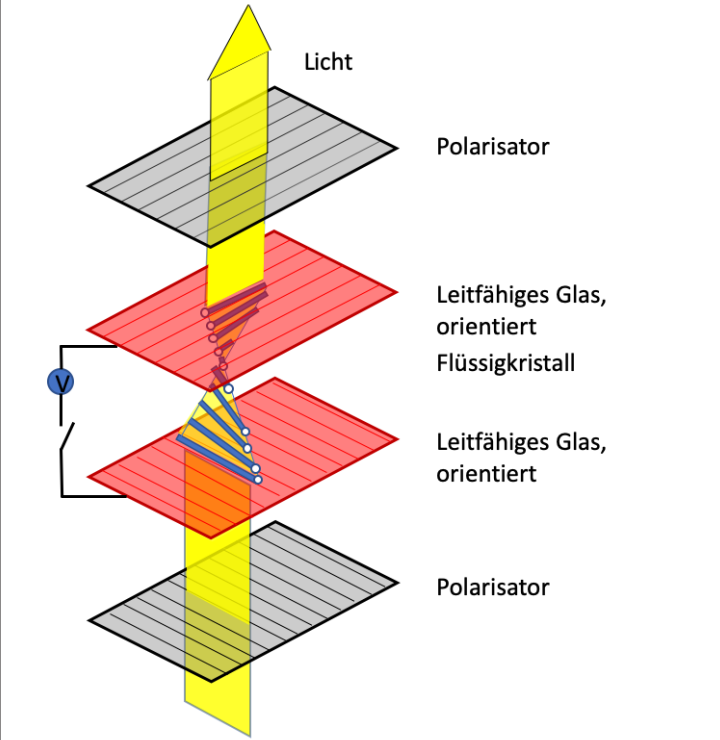
\includegraphics[width=0.7\linewidth]{images/TN-Zelle1.png}
		
		ohne angelegte Spannung   
	\end{center}
\end{minipage}
\hfill
\begin{minipage}{0.45\linewidth}
	\begin{center}
		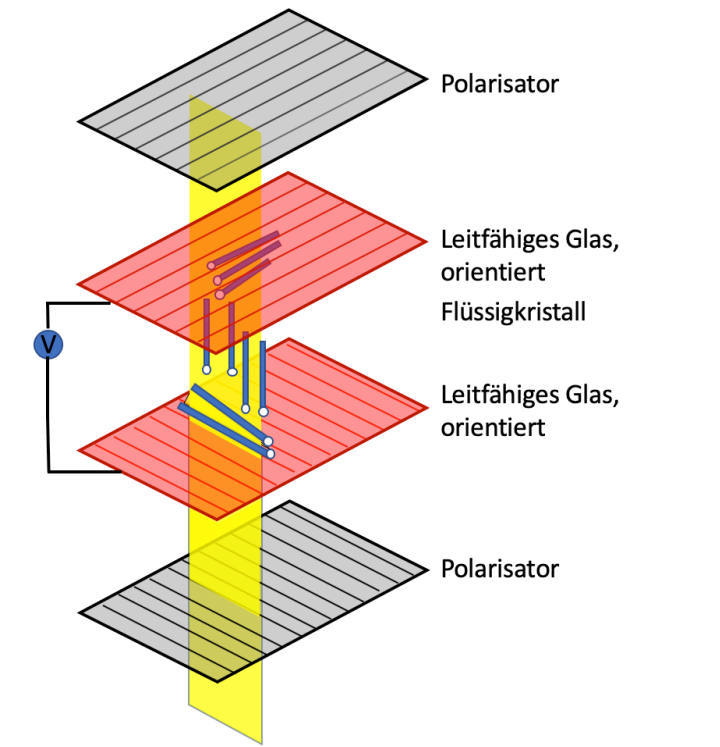
\includegraphics[width=0.7\linewidth]{images/TN-Zelle2.png} 
		
		mit angelegter Spannung 
	\end{center}
\end{minipage}
